%% LyX 2.2.0 created this file.  For more info, see http://www.lyx.org/.
%% Do not edit unless you really know what you are doing.
\documentclass[12pt,hyperfootnotes=false]{article}
\usepackage{mathptmx}
\usepackage[latin9]{inputenc}
\usepackage{geometry}
\geometry{verbose,tmargin=1in,bmargin=1in,lmargin=1in,rmargin=1in}
\usepackage{float}
\usepackage{amsmath}
\usepackage{amsthm}
\usepackage{amssymb}
\usepackage{graphicx}
\usepackage{setspace}
\usepackage[authoryear]{natbib}
\onehalfspacing
\usepackage[unicode=true]
 {hyperref}

\makeatletter
%%%%%%%%%%%%%%%%%%%%%%%%%%%%%% Textclass specific LaTeX commands.
 \theoremstyle{definition}
 \newtheorem*{defn*}{\protect\definitionname}

%%%%%%%%%%%%%%%%%%%%%%%%%%%%%% User specified LaTeX commands.
\usepackage{amsthm}
\usepackage{bm}
\usepackage{setspace}
\usepackage{sectsty}

\usepackage{datetime}
\usepackage{pdflscape}
\usepackage[english]{babel}
\usepackage{times}
\usepackage[small]{caption}
\usepackage[bottom,hang,flushmargin]{footmisc}

\DeclareMathOperator{\sgn}{sgn}
\DeclareMathOperator{\Var}{Var}
\DeclareMathOperator{\Corr}{Corr}
\DeclareMathOperator{\Cov}{Cov}
\DeclareMathOperator{\E}{E}
\DeclareMathOperator{\logit}{logit}
\DeclareMathOperator{\I}{I}

\sectionfont{\noindent\normalfont\large\bf}
\subsectionfont{\noindent\normalfont\normalsize\bf}
\subsubsectionfont{\noindent\normalfont\it}

\pdfminorversion=4

\makeatother

  \providecommand{\definitionname}{Definition}

\begin{document}

\title{\noindent \textbf{Paper}}

\author{\noindent Matthew Gentzkow,\textbf{ }\textit{Stanford University}\textbf{}\thanks{E-mail:\ gentzkow@stanford.edu, jesse\_shapiro\_1@Brown.edu. Acknowledgements
here.}\textbf{}\\
Jesse M. Shapiro, \textit{Brown University} \textbf{}\\
}

\date{\monthname\ \number\year}
\maketitle
\begin{abstract}
\noindent The abstract.

\bigskip{}
\end{abstract}
\pagebreak{}

\begin{spacing}{1.4}

\section{Introduction}

This is a sample introduction.\footnote{This is a sample footnote. } 

\section{Data\label{sec:data}}

Data description here. 

\section{Model\label{sec:model}}

\subsection{Probability model\label{subsec:prob-model}}

This is the first model section. Below is some inserted math.
\begin{equation}
{\bf x}_{t}\sim\text{{N}}\left(0,1\right),\label{eq:multinomial}
\end{equation}
where $\mathbf{x}_{t}$ is a random variable.

\subsection{Other model subsection.\label{subsec:cmodel_subsection}}

Other model information goes here. 
\begin{defn*}
You can place a definition here. 
\end{defn*}

\section{Estimation\label{sec:estimation}}

This is the estimation section.

\section{Results\label{sec:results}}

Figure \ref{fig:plot} is a sample figure. 

\section{Discussion\label{sec:Discussion}}

This is a discussion.

\section{Conclusion}

This is the conclusion.

\end{spacing}

\pagebreak{}

\section*{References}

\leftskip=2em 
\parindent=-2em
\onehalfspacing

\noindent

Gentzkow, Matthew and Jesse M. Shapiro. 2010. What drives media slant?
Evidence from U.S. daily newspapers. \textit{Econometrica} 78(1):
35\textendash 71.

Gentzkow, Matthew, Jesse M. Shapiro, and Matt Taddy. 2015. Measuring
polarization in high-dimensional data: Method and application to Congressional
speech. Stanford University mimeo. Accessed at \\
$<$\href{http://web.stanford.edu/~gentzkow/research/politext.pdf}{http://web.stanford.edu/$\sim$gentzkow/research/politext.pdf}$>$
on July 6, 2016.

\parindent=2em
\leftskip=0em

\pagebreak{}


\appendix
\begin{center}
\textbf{\LARGE{}Appendices}
\par\end{center}{\LARGE \par}

\section{Table appendix\label{sec:table_appendix}}

This appendix links to tables and is followed by links to figures. 

\newpage{}

\begin{figure}[H]
\begin{centering}
\caption{Plot \label{fig:plot}}
\par\end{centering}
\begin{centering}
\emph{\smallskip{}
}
\par\end{centering}
\centering{}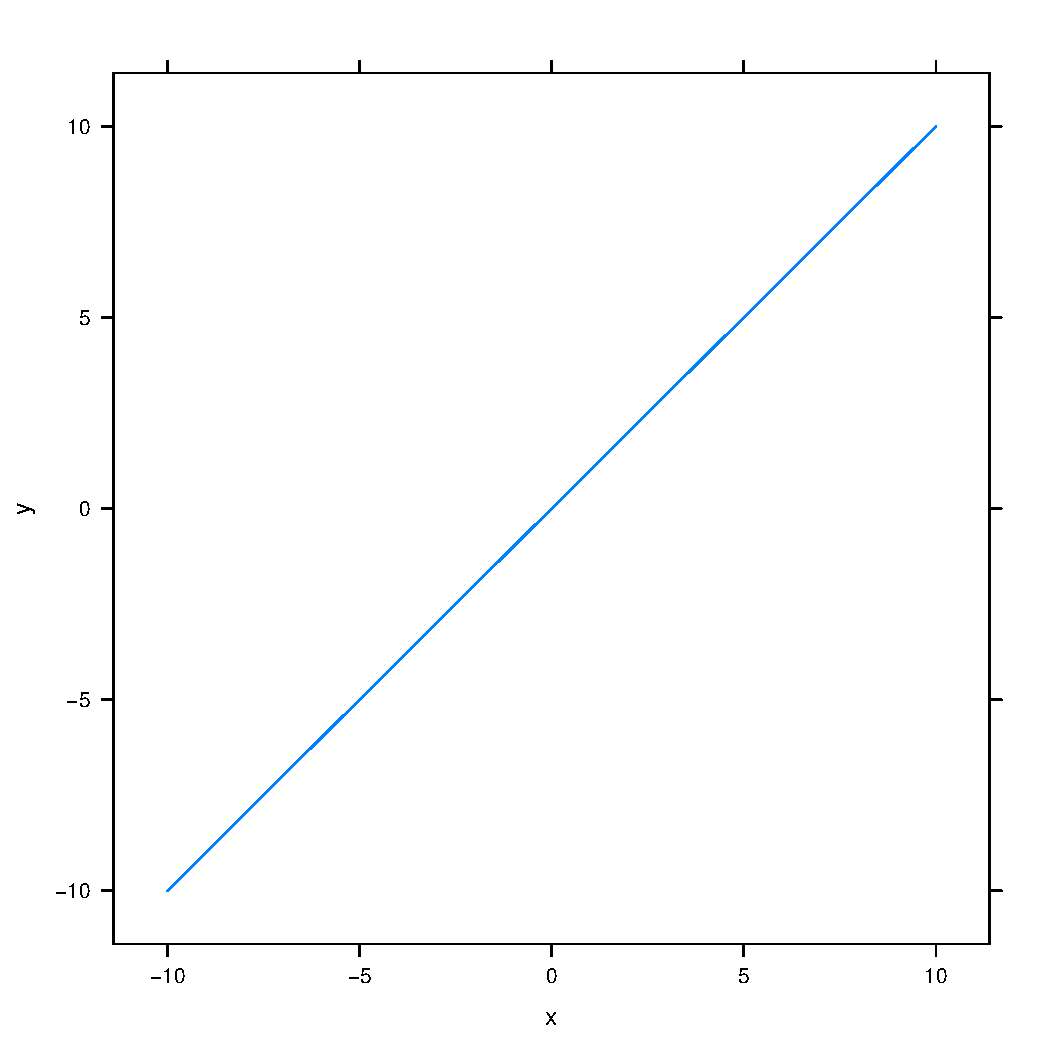
\includegraphics[scale=0.75]{../../output/analysis/example/plot}
\end{figure}

\clearpage

\begin{figure}[H]
{\small{}\caption*{Appendix Figure: Subtitle}}\label{fig:variants}

\medskip{}

\begin{centering}
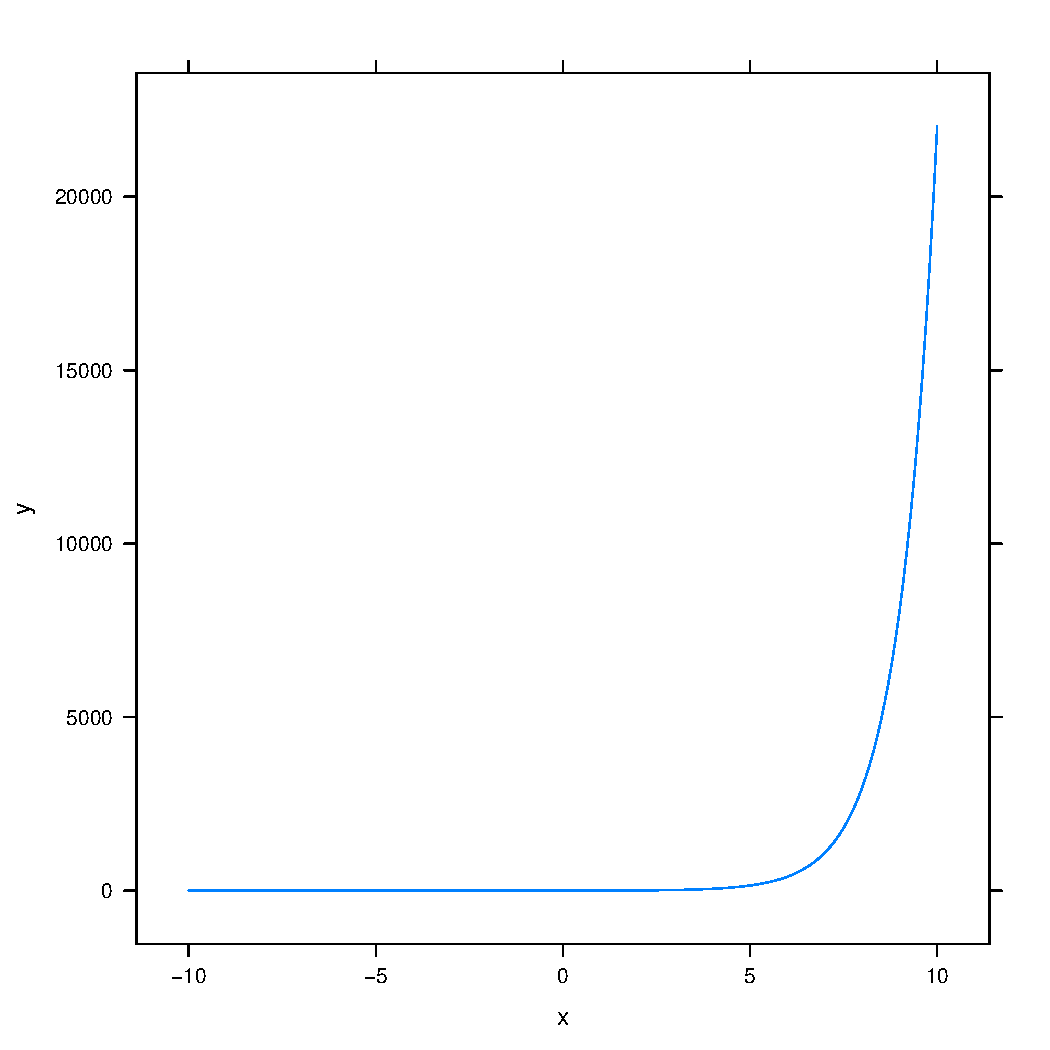
\includegraphics[width=1\textwidth]{../../output/analysis/example/appendix_plot}
\par\end{centering}
\begin{centering}
\smallskip{}
\par\end{centering}
{\small{}Notes: }{\small \par}
\end{figure}

\newpage{}


\renewcommand{\figurename}{Appendix Figure}
\setcounter{figure}{0}
\end{document}
